% vim: set textwidth=120:

% Example CV based on the 1.5-column-cv template. Main features:
% * uses the Roboto font family and IcoMoon icon set;
% * doesn't use colours, different font weights are used instead for styling;
% * because the CV fits on one page, header and footer is empty, since there isn't much useful info to put there;
% * includes a photo.
\documentclass[a4paper,10pt]{article}


% package imports
% ---------------

\usepackage[british]{babel} % for correct language and hyphenation and stuff
\usepackage{calc}           % for easier length calculations (infix notation)
\usepackage{enumitem}       % for configuring list environments
\usepackage{fancyhdr}       % for setting header and footer
\usepackage{fontspec}       % for fonts
\usepackage{geometry}       % for setting margins (\newgeometry)
\usepackage{graphicx}       % for pictures
\usepackage{microtype}      % for microtypography stuff
\usepackage{xcolor}         % for colours
\usepackage[utf8]{inputenc}
% use KoTeX package for Korean 
\usepackage{kotex}

% margin and column widths
% ------------------------


% margins
\newgeometry{left=15mm,right=15mm,top=15mm,bottom=15mm}

% width of the gap between left and right column
\newlength{\cvcolumngapwidth}
\setlength{\cvcolumngapwidth}{3.5mm}

% left column width
\newlength{\cvleftcolumnwidth}
\setlength{\cvleftcolumnwidth}{44.5mm}

% right column width
\newlength{\cvrightcolumnwidth}
\setlength{\cvrightcolumnwidth}{\textwidth-\cvleftcolumnwidth-\cvcolumngapwidth}

% set paragraph indentation to 0, because it screws up the whole layout otherwise
\setlength{\parindent}{0mm}


% style definitions
% -----------------
% style categories explanation:
% * \cvnameXXX is used for the name;
% * \cvsectionXXX is used for section names (left column, accompanied by a horizontal rule);
% * \cvtitleXXX is used for job/education titles (right column);
% * \cvdurationXXX is used for job/education durations (left column);
% * \cvheadingXXX is used for headings (left column);
% * \cvmainXXX (and \setmainfont) is used for main text;
% * \cvruleXXX is used for the horizontal rules denoting sections.

% font families
\defaultfontfeatures{Ligatures=TeX} % reportedly a good idea, see https://tex.stackexchange.com/a/37251

\newfontfamily{\cvnamefont}{KoPubWorld Dotum Bold.ttf}
\newfontfamily{\cvsectionfont}{Roboto-Medium.ttf}
\newfontfamily{\cvtitlefont}{KoPubWorld Dotum Bold.ttf}
\newfontfamily{\cvdurationfont}{Roboto-LightItalic.ttf}
\newfontfamily{\cvheadingfont}{Roboto-Regular.ttf}
\newfontfamily{\cvimportant}{KoPubWorld Dotum Bold.ttf}
%\newfontfamily{\cvHangul}{KoPubWorld Dotum Bold.ttf}
%\setmainfont{Roboto-Light.ttf}
\setmainfont{KoPubWorld Dotum Light.ttf}

% colours
\definecolor{cvnamecolor}{HTML}{000000}
\definecolor{cvsectioncolor}{HTML}{000000}
\definecolor{cvtitlecolor}{HTML}{000000}
\definecolor{cvdurationcolor}{HTML}{000000}
\definecolor{cvheadingcolor}{HTML}{000000}
\definecolor{cvmaincolor}{HTML}{000000}
\definecolor{cvrulecolor}{HTML}{000000}

\color{cvmaincolor}

% styles
\newcommand{\cvnamestyle}[1]{{\Large\cvnamefont\textcolor{cvnamecolor}{#1}}}
\newcommand{\cvsectionstyle}[1]{{\normalsize\cvsectionfont\textcolor{cvsectioncolor}{#1}}}
\newcommand{\cvtitlestyle}[1]{{\large\cvtitlefont\textcolor{cvtitlecolor}{#1}}}
\newcommand{\cvdurationstyle}[1]{{\small\cvdurationfont\textcolor{cvdurationcolor}{#1}}}
\newcommand{\cvheadingstyle}[1]{{\normalsize\cvheadingfont\textcolor{cvheadingcolor}{#1}}}


% inter-item spacing
% ------------------

% vertical space after personal info and standard CV items
\newlength{\cvafteritemskipamount}
\setlength{\cvafteritemskipamount}{5mm plus 1.25mm minus 1.25mm}

% vertical space after sections
\newlength{\cvaftersectionskipamount}
\setlength{\cvaftersectionskipamount}{2mm plus 0.5mm minus 0.5mm}

% extra vertical space to be used when a section starts with an item with a heading (e.g. in the skills section),
% so that the heading does not follow the section name too closely
\newlength{\cvbetweensectionandheadingextraskipamount}
\setlength{\cvbetweensectionandheadingextraskipamount}{1mm plus 0.25mm minus 0.25mm}


% intra-item spacing
% ------------------

% vertical space after name
\newlength{\cvafternameskipamount}
\setlength{\cvafternameskipamount}{3mm plus 0.75mm minus 0.75mm}

% vertical space after personal info lines
\newlength{\cvafterpersonalinfolineskipamount}
\setlength{\cvafterpersonalinfolineskipamount}{2mm plus 0.5mm minus 0.5mm}

% vertical space after titles
\newlength{\cvaftertitleskipamount}
\setlength{\cvaftertitleskipamount}{1mm plus 0.25mm minus 0.25mm}

% value to be used as parskip in right column of CV items and itemsep in lists (same for both, for consistency)
\newlength{\cvparskip}
\setlength{\cvparskip}{0.5mm plus 0.125mm minus 0.125mm}

% set global list configuration (use parskip as itemsep, and no separation otherwise)
\setlist{parsep=0mm,topsep=0mm,partopsep=0mm,itemsep=\cvparskip}


% CV commands
% -----------

% creates a "personal info" CV item with the given left and right column contents, with appropriate vertical space after
% @param #1 left column content (should be the CV photo)
% @param #2 right column content (should be the name and personal info)
\newcommand{\cvpersonalinfo}[2]{
    % left and right column
    \begin{minipage}[t]{\cvleftcolumnwidth}
        \vspace{0mm} % XXX hack to align to top, see https://tex.stackexchange.com/a/11632
        \raggedleft #1
    \end{minipage}% XXX necessary comment to avoid unwanted space
    \hspace{\cvcolumngapwidth}% XXX necessary comment to avoid unwanted space
    \begin{minipage}[t]{\cvrightcolumnwidth}
        \vspace{0mm} % XXX hack to align to top, see https://tex.stackexchange.com/a/11632
        #2
    \end{minipage}

    % space after
    \vspace{\cvafteritemskipamount}
}

% typesets a name, with appropriate vertical space after
% @param #1 name text
\newcommand{\cvname}[1]{
    % name
    \cvnamestyle{#1}

    % space after
    \vspace{\cvafternameskipamount}
}

% typesets a line of personal info beginning with an icon, with appropriate vertical space after
% @param #1 parameters for the \includegraphics command used to include the icon
% @param #2 icon filename
% @param #3 line text
\newcommand{\cvpersonalinfolinewithicon}[3]{
    % icon, vertically aligned with text (see https://tex.stackexchange.com/a/129463)
    \raisebox{.5\fontcharht\font`E-.5\height}{\includegraphics[#1]{#2}}
    % text
    #3

    % space after
    \vspace{\cvafterpersonalinfolineskipamount}
}

% creates a "section" CV item with the given left column content, a horizontal rule in the right column, and with
% appropriate vertical space after
% @param #1 left column content (should be the section name)
\newcommand{\cvsection}[1]{
    % left and right column
    \begin{minipage}[t]{\cvleftcolumnwidth}
        \raggedleft\cvsectionstyle{#1}
    \end{minipage}% XXX necessary comment to avoid unwanted space
    \hspace{\cvcolumngapwidth}% XXX necessary comment to avoid unwanted space
    \begin{minipage}[t]{\cvrightcolumnwidth}
        \textcolor{cvrulecolor}{\rule{\cvrightcolumnwidth}{0.3mm}}
    \end{minipage}

    % space after
    \vspace{\cvaftersectionskipamount}
}

% creates a standard, multi-purpose CV item with the given left and right column contents, parskip set to cvparskip
% in the right column, and with appropriate vertical space after
% @param #1 left column content
% @param #2 right column content
\newcommand{\cvitem}[2]{
    % left and right column
    \begin{minipage}[t]{\cvleftcolumnwidth}
        \raggedleft #1
    \end{minipage}% XXX necessary comment to avoid unwanted space
    \hspace{\cvcolumngapwidth}% XXX necessary comment to avoid unwanted space
    \begin{minipage}[t]{\cvrightcolumnwidth}
        \setlength{\parskip}{\cvparskip} #2
    \end{minipage}

    % space after
    \vspace{\cvafteritemskipamount}
}

% typesets a title, with appropriate vertical space after
% @param #1 title text
\newcommand{\cvtitle}[1]{
    % title
    \cvtitlestyle{#1}

    % space after
    \vspace{\cvaftertitleskipamount}
    % XXX need to subtract cvparskip here, because it is automatically inserted after the title "paragraph"
    \vspace{-\cvparskip}
}


% header and footer
% -----------------

% set empty header and footer
\pagestyle{empty}


% preamble end/document start
% =========================== BEGIN ===========================

\begin{document}


% personal info
% -------------

\cvpersonalinfo{
    % photo
    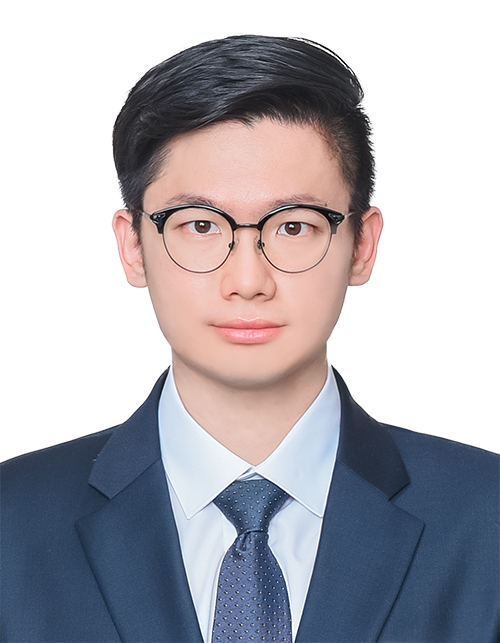
\includegraphics[height=45mm]{Hyeonjun02.jpg}
}{
    % name
    \cvname{\Huge 박  현  준}

    % address
%    \cvpersonalinfolinewithicon{height=4mm}{072-location.pdf}{
%        Flat Number 40, Anupam Apartment, Vasundhara Enclave, Delhi-110096
%    }

    % phone number
    \cvpersonalinfolinewithicon{height=5mm}{067-phone.pdf}{
        +82 10-4037-8702
    }

    % email address
    \cvpersonalinfolinewithicon{height=5mm}{070-envelop.pdf}{
        koreaphj91@gmail.com
    }

    % LinkedIn account
    \cvpersonalinfolinewithicon{height=5mm}{458-linkedin.pdf}{
        https://www.linkedin.com/in/hyeonjun-park-41bb59125/
    }
    
    % Github account
    \cvpersonalinfolinewithicon{height=5mm}{github.png}{
        https://github.com/MrLacquer?tab=repositories
    }
    
    % google scholar account
    \cvpersonalinfolinewithicon{height=5mm}{google_scholar.png}{
        https://bit.ly/2FQS02U
    }
}


%%%% work experience
% ---------------
%\cvsection{WORK EXPERIENCE}

%%%% Fake Company 2
%\cvitem{
%    \cvdurationstyle{January 2019 -- present}
%}{
%    \cvtitle{Graduate Engineer Trainee}
%
%    NEC Technologies Pvt. Ltd., Sector 135, Noida, Uttar Pradesh
%
%    \begin{itemize}[leftmargin=*]
%        \item Working on Openshift, Kubernetes, GoLang and Openstack.
%    \end{itemize}
%}


% education
% ---------
\vspace*{1cm}

\cvsection{EDUCATION}

% Ph.D's
\cvitem{
    \cvdurationstyle{Mar. 2016 -- Present}
}{
    \cvtitle{Ph.D in Engineering (예정) (전자공학과)}
    경희대학교 (경기도 용인시 기흥구)
    \begin{itemize}[leftmargin=*]
        \item 학위논문: Development of Anthropomorphic Robot Hand for Adaptive Variable Grasping Stiffness
        \item 지도교수: 김 동 한
    \end{itemize}
}

% Master's
\cvitem{
    \cvdurationstyle{Mar. 2014 -- Feb. 2016}
}{
    \cvtitle{Master in Engineering (전자 전파공학과)}
    경희대학교 (경기도 용인시 기흥구)
    \begin{itemize}[leftmargin=*]
        \item 학위논문: 바이올린 운지법을 위한 의인화형 로봇손 개발 
        \newline (영문명: Development of Anthropomorphic Robot Hand for Violin Fingering)
        \item 지도교수: 김 동 한
    \end{itemize}
}

% bachelor's
\cvitem{
    \cvdurationstyle{Mar. 2010 -- Feb. 2014}
}{
    \cvtitle{Bachelor in Engineering (로봇공학과, \textbf{Summa cum laude})}
    호서대학교 (충청남도 아산시)
    \begin{itemize}[leftmargin=*]
        \item 학위논문: 줄 꼬임 기반 구동 로봇 손과 데이터 장갑을 이용한 제어 
        \newline (영문명: Using gloves, motion control of a string twist-based robot hand)
        \item 지도교수: 류 근 호
    \end{itemize}
}

% skills
% ------


\vspace*{1cm}

\cvsection{Technical skills}

\vspace{\cvbetweensectionandheadingextraskipamount}

\cvitem{
    \cvheadingstyle{Computer Languages}
}{
    \begin{itemize}
    \item Python
    \item C\#
    \item C/C++
    \item MATLAB
    \item ROS(Robot Operating System)
            
    \end{itemize}
}
\cvitem{
    \cvheadingstyle{Design Program}
}{
    \underline{for 3D design}
    \begin{itemize}
        \item Fusion 360 (Auto Desk Co.)
        \item Creo (Pro/E)
        \item Solidworks
    \end{itemize}
    
    \underline{for 2D design}
    \begin{itemize}
        \item Auto CAD
    \end{itemize}
    
    \underline{for PCB artwork design (ECAD)}
    \begin{itemize}
        \item Altium Designer
    \end{itemize}
    
}

\cvitem{
    \cvheadingstyle{Micro-controller}
}{
    \begin{itemize}
        \item ARM Cortex-M (32bit processor)
        \item Arduino
        \item Atmega, PIC (8bit processor)
    \end{itemize}
}
%----------------------------------------------------------------------------------------
%	WORK EXPERIENCE SECTION
%----------------------------------------------------------------------------------------
\newpage
\cvsection{Professional Experience}

\vspace{\cvbetweensectionandheadingextraskipamount}

\cvitem{
    \cvdurationstyle{Mar. 2014 -- Present}
}{
    \cvtitle{연구원 (경희대학교)}
    \item \underline{\textbf{Human and Robot Interaction (HRI) Lab.(formal Auto Control Lab.)}}
    \begin{enumerate}
        %------------------------------------------------ HRI; Ph. D candidate
        \item 적응형 가변식 파지강성을 위한 의인화형 로봇 손 개발: 
        \begin{itemize}
            \item 물체의 탄성에 순응하여 파지 강성이 능동적으로 조절되는 임피던스 제어 기반의 의인화형 로봇 손 개발 
            \item 두 개의 4절 링크 구조를 결합, under-actuated 메커니즘기반의 로봇 손가락 모듈 설계.
            \item 로봇 손의 외력을 감지하기 위해서 fingertip force sensor 및 SEA (Series Elastic Actuator) module을 적용함.
            \item 로봇 손을 동작 시키는 전기적 회로, impedance 제어기 등을 설계함.
        \end{itemize}
        \item 근력 증강 로봇의 sEMG 센서 신호 처리를 위한 모듈 및 제어 아키텍쳐 개발 참여:
        \begin{itemize}
            \item 2018.09 - 2019.08, 한국산업평가관리원 
            \item 프로젝트 명: 근력증강로봇 제어를 위한 피부부착형 다중센서 통합모듈 및 강건한 운동의도 명령 생성기술 개발
            \item 담당 업무:
                \begin{itemize}
                    \item 근력 증강 로봇의 제어를 위한 생체 신호(sEMG) 및 물리 센서의 회로 및 상보필터 개발
                    \item 근력증강로봇 제어를 위한 피부부착형 다중 센서 중, 증폭된 EMG 신호 회로와 24bit A/D Converter칩 간의 회로 구성
                    \item 24bit A/DC과 마이크로프로세서(MCU) 간의 SPI 통신 회로 구성 및 프로토콜 분석
                    \item 설계된 아날로그 회로의 PCB 설계
                \end{itemize}
        \end{itemize}
        \item 개인용 탑승 로봇의 안정성 평가를 위한 동적 더미 시스템 개발 참여:
        \begin{itemize}
            \item 2018.09 - 2019.08, 한국산업평가관리원
            \item 프로젝트 명: 개인지원 로봇의 안전성(ISO 13482) 인증을 위한 시험평가 기술 및 인증 프로세스 통합 플랫폼 개발
            \item 담당 업무:
                \begin{itemize}
                    \item 동적 더미 시스템 구현을 위한 6 motor 기반의 stweart platform 설계
                    \item 설계한 stweart platform의 역기구학 해석 및 제어 시스템 구현
                \end{itemize}
        \end{itemize}
        
        \item 양팔 로봇 기반의 바이올린 연주 로봇 시스템 개발:
        \begin{itemize}
            \item 2016.11-2019.10, 한국연구재단(학술진흥)
            \item 프로젝트 명: 음악을 통한 인간과 로봇간의 교감(HRI)을 위한 인공감성 청각 모델 기술 개발
            \item 담당 업무:
                \begin{itemize}
                    \item 인공감성 청각 모델 검증을 위한 바이올린 연주 로봇 시스템 구성
                    \item 두 개의 상용 로봇 팔을 기반으로 양팔 로봇의 설계, ROS 패키지 개발 및 제어 시스템을 개발 함.
                    \item 임베디드 시스템의 관리를 위한 C# dot Net UI 프로그램 개발
                    \item 인공감성 청각 모델 검증을 위한 소리 분석 시스템 구성 및 펌웨어를 개선함 (기존 대비 2배 성능 상향).
                \end{itemize}
        \end{itemize}
        % 한화 1.5억원, 1억원
        \item 기타 사항:
        \begin{itemize}
            \item 국가과제 제안서 작성 참여(도합 12.2억원 규모): 
            \newline 한국연구재단(2016R1D1A1A02936946), 산업기술평가원(10080348)
        \end{itemize}
    \end{enumerate}
}

\cvitem{
    \cvdurationstyle{May. 2020 -- Dec. 2020}
}{
    \cvtitle{연구원 (명지대학교)} 
    \item \underline{\textbf{IRS(Intelligent Robot System) Lab.}}
    \begin{enumerate}[leftmargin=*]
        \item IRS LAB 휴머노이드 로봇의 파워 보드 설계 참여:
        \begin{itemize}
            \item 2020.05 - 2020.12, 한국연구재단(학술진흥)
            \item 프로젝트 명: 다축 로봇의 물리 파라미터 추정 시스템 개발
                \begin{itemize}
                    \item 휴머노이드 로봇의 파워보드 PCB artwork 설계 및 검증 실험을 진행함.
                \end{itemize}
        \end{itemize}
    \end{enumerate}
}

\cvitem{
    \cvdurationstyle{Jul. 2018 -- Aug. 2018}
}{
    \cvtitle{방문연구원 (in Purdue University, USA)} 
    \item \underline{\textbf{Purdue SMART Lab.}}
    \begin{enumerate}[leftmargin=*]
        \item 생체신호처리를 위한 core module 개발:
        \begin{itemize}
            \item 생체신호(sEMG) 신호를 처리하기 위한 고성능 Micro-controller 보드를 설계함 (기존 대비 120\% 향상 시킴).
            \item 모든 기능들이 강건하게 작동 될 수 있도록 전원 노이즈를 최소화 시켜서 설계함.
        \end{itemize}
    \end{enumerate}
}


\cvitem{
    \cvdurationstyle{Mar. 2012 -- Feb. 2013}
}{
    \cvtitle{학부연구원 (호서대학교)}
    \underline{\textbf{Robot for Human (R4H) Lab.}}
    \begin{enumerate}[leftmargin=*]
        \item 모터 제어 시스템 교육 자료 개발 참여:
        \begin{itemize}
            \item Micro-controller와 다양한 센서를 이용하여 모터를 제어 할 수 있도록 하는 교육용 자료를 제작함.
        \end{itemize}
        \item 외주 계약 프로젝트 참여: 
        \begin{itemize}
            \item Robotis 회사의 교육용 로봇 플랫폼인 "STEM standard \& expansion version"을 C언어로 개발하여 납품함.
        \end{itemize}
    \end{enumerate}
}

\cvitem{
    \cvdurationstyle{Sep. 2011 -- Jun. 2012}    
}{
    \underline {\textbf{Department of Robotics Engineering}}
    \begin{enumerate}[leftmargin=*]
        \item 교육용 2족 로봇 플랫폼 및 휴머노이드 로봇 설계 및 개발 참여
        \item Teaching Assistance: How to make 2D\&3D modeling for sophomore of the department of Robotics
    \end{enumerate}
    }

% Award Section
\cvsection{Awards and Honors}

\vspace{\cvbetweensectionandheadingextraskipamount}

\cvitem{
    \cvheadingstyle{Oct. 2012}
}{
    \cvtitle{1st Place Award of Useful Idea Prize (in Hoseo University)}
    \begin{itemize}
        \item The Capstone Design Contest -- Development of Armadillo Biomimetic Mobile Robot System
       
    \end{itemize}
}
\cvitem{
    \cvheadingstyle{July. 2012, Oct. 2011}
}{
    \cvtitle{The Best Mentor Award (in Hoseo University)}
    \begin{itemize}
        \item Programming and teaching how to control motor with various sensors using micro controller unit
        \item Teaching how to make 2D\&3D modeling for sophomore of the department of Robotics
    \end{itemize}
}
\cvitem{
    \cvheadingstyle{from 2010 to 2013}
}{
    \cvtitle{Academic Scholarships (in Hoseo University)}
    \begin{itemize}
        \item Awarded to the student for obtaining an outstanding GPA by Hoseo University from 2010 to 2013
    \end{itemize}
}

\vspace*{1cm}

% Publications
\cvsection{Publications}

%\vspace{\cvbetweensectionandheadingextraskipamount}

\cvitem{
    \cvheadingstyle{Journals}
}{
    \begin{itemize}
    \item Harin Kim, {\cvimportant Hyeonjun Park}, Sangheum Lee, Donghan Kim, "Joint Torque Estimation Using sEMG and Deep Neural Network", {\em Journal of Electrical Engineering & Technology}, 1 (1), pp. 1-12, 2020.  {\cvimportant SCIE, IF 0.736}
    \item {\cvimportant Hyeonjun Park}, Donghan Kim, "An open-source anthropomorphic robot hand system: HRI hand", {\em HardwareX}, e00100, pp. 1-12, 2020.  
    \item {\cvimportant Hyeonjun Park}, Bumjoo Lee and Donghan Kim, "Development of Anthropomorphic Robot Finger for Violin Fingering", Journal of Electronics and Telecommunications Research Institute, 38 (6), pp. 1218-1228, 2016. {\cvimportant SCI, IF 1.094} 
    \item {\cvimportant Hyeonjun Park}, Bumjoo Lee and Donghan Kim, "Violin Musical Tone Analysis Using Robot Finger", {\em Procedia Computer Science}, 94 (1), pp.398-403, 2016.
    \item Hwon-Jae Jung, {\cvimportant Hyeonjun Park} and Donghan Kim, "Improvement of Gesture Recognition using 2-stage HMM", {\em Journal of Institute of Control, Robotics and Systems}, 21 (11), pp. 1034-1037, 2015.
    \item {\cvimportant Hyeonjun Park}, Wonse Jo, Kyeongmin Choi and Donghan Kim, "A Study about Robotic Hand and Finger for Violin Playing Robot", {\em International Journal of Applied Engineering Research}, 10 (11), pp. 27553-27557, 2015.
    \item {\cvimportant Hyeonjun Park}, Wonse Jo, Kyeongmin Choi, Hwonjae Jung, Bum-Joo Lee and Donghan Kim, "A Study about Sound Quality for Violin Playing Robot", {\em Procedia Computer Science}, 56 (1), pp. 496-501, 2015.        
            
    \end{itemize}
}

\cvitem{
    \cvheadingstyle{Conference}
}{
    \begin{itemize}
    \item {\cvimportant Hyeonjun Park}, Bumjoo Lee, Donghan Kim, "Design of Modular End-effector for Collaborative Robot based on Underactuated Mechanism", 2020 Fourth IEEE International Conference on Robotic Computing (IRC), pp. 488-492, Nov. 2020.
    \item Sangheum Lee, {\cvimportant Hyeonjun Park}, Harin Kim, Taeyang Gwon, Donghan Kim, "Real-Time Joint Torque Estimation on Embedded system using EMG and Artificial Neural Network for Exoskeleton Robot", 2020 Fourth IEEE International Conference on Robotic Computing (IRC), pp. 483-487, Nov. 2020.
    \item {\cvimportant Hyeonjun Park}, Donghan Kim, "Development of ROS-based Integrated Control System for Cooperative Robot with Anthropomorphic Robot Hand", {\em 2020 IEIE(Institute of Electronics and Information Engineers) summer annual conference}, pp. 1476-1480, 2020.
    \item {\cvimportant Hyeonjun Park}, Donghan Kim, "Design and Control of an Anthropomorphic Type Robot Finger based on Series Elastic Actuator Module", {\em 2020 ICROS(Institute of Control, Robotics and Systems) annual conference}, pp. 279-280, 2020.
    \item Sangheum Lee, {\cvimportant Hyeonjun Park}, Harin Kim, Bumjoo Lee, Donghan Kim, "Joint Torque Estimation based on ANN for Exoskeleton robot through Complementary filtering of EMG and Torque sensor", {\em 2020 ICROS(Institute of Control, Robotics and Systems) annual conference}, pp. 328-329, 2020.
    \item Taeyang Gwon, {\cvimportant Hyeonjun Park}, Sanghuem Lee, Donghan Kim, "Development of a Dynamic Dummy System to Describe Human Waist Movement for Safety Evaluation of Person Carrier Robot", {\em 2020 IEIE(Institute of Electronics and Information Engineers) summer annual conference}, pp. 1626-1631, 2020.
    \item Sangheum Lee, {\cvimportant Hyeonjun Park}, Donghan Kim, "Integrated control algorithm for mobile manipulator system using artificial neural network", {\em 2020 IEIE(Institute of Electronics and Information Engineers) summer annual conference}, pp. 1509-1513, 2020.
    \item TaeYang Gwon, {\cvimportant Hyeonjun Park}, DongHyeon Seo, Sangheum Lee, Sangwon Jeon and Donghan Kim, "A Study on Safety Evaluation Criteria of the Personal Carrier  Robot based on ISO 13482", {\em 2019 Third IEEE International Conference on Robotic Computing}, pp.1-5, 2019.         
    \item {\cvimportant Hyeonjun Park}, Donghan Kim, "Force analysis using finger dummy for violin fingering", {\em 2018 IEEE Sensors Applications Symposium(SAS)}, pp.1-5, 2018.
    \item Eunha Moon, {\cvimportant Hyeonjun Park} and Donghan Kim, "Development of Robot Hand focused on Violin Fingering", {\em 2018 Second IEEE International Conference on Robotic Computing} , pp.342-346, 2018.
    \item {\cvimportant Hyeonjun Park}, Bumjoo Lee and Donghan Kim, "A Study on Modular Design of End Effector", {\em International Workshop on Robot Modularity in conjunction with International Conference on Intelligent Robots and Systems(IROS)}, pp. 1-4, 2016.
    \item {\cvimportant Hyeonjun Park}, Bumjoo Lee and Donghan Kim, "Development of Anthropomorphic Robot hand built-in 3-Axis Load cell", {\em 2015 KSMTE(Korean Society of Manufacturing Technology Engineers) annual autumn conference}, pp. 14-14, 2015. 
    \item Hwon-Jae Jung, {\cvimportant Hyeonjun Park} and Donghan Kim, "Gesture Recognition with IMU and EMG sensors by using 2-stage HMM", {\em 2015 ICROS(Institute of Control, Robotics and Systems) annual conference}, pp. 179-180, 2015.
    \item Wonse Jo, {\cvimportant Hyeonjun Park}, Bumjoo Lee, Donghan Kim, "A study on improving sound quality of violin playing robot", {\em 2015 6th ICARA(International Conference on Automation, Robotics and Applications)}, pp. 185-191, 2015.
    \item Seong-Og Shin, {\cvimportant Hyeonjun Park}, Donghan Kim, "Gesture based Communication between Human and Heterogeneous Robots", {\em 2014 ICROS(Institute of Control, Robotics and Systems) annual conference}, pp. 408-409, 2014.
    \item Keun-Ho REW, {\cvimportant Hyeonjun Park}, Eunha Moon, Hyuk Woo KWON, Jun Hyeok HAM, "C Pro-gramming Education through Robots", {\em The Korean society of mechanical engineers annual autumn conference}, pp.1388-1391, 2012.

    \end{itemize}
}

\cvitem{
    \cvheadingstyle{Patents}
}{
    
    \begin{itemize}
    \item {\cvimportant 박현준}, 김동한, ”모듈화 기반의 링크 구조 로봇 손가락”, 출원번호 10-2019-0137152, October 2019.
    \item 이상흠, {\cvimportant 박현준}, 김동한, ”다채널 근전도 신호측정을 통한 딥러닝 기반 관절토크 추정 시스템”, 출원번호 No. 10-2019-0141365, November 2019.
    \item 이상흠, {\cvimportant 박현준}, 김하린, 김동한, ” 팔꿈치의 회전 운동에 대한 관절 토크 측정 시스템”, 출원번호 No. 10-2019-0141367, November 2019.
    \item 김진현, 강석범, 김동한, {\cvimportant 박현준}, 김하린, 강연, “인솔형 보행 분석 장치”, 출원번호 No. 10-2017-0172844, December 2017.
    \item {\cvimportant 박현준}, 김동한, ”자기공진방식을 활용한 충전 드론”, 등록번호 10-1812234, December 2017.
    \item {\cvimportant 박현준}, 김동한, 자기공진방식을 이용한 드론 충전시스템 및 제어방법, 등록번호 No. 10-1812234, December 2017.
    \item 김동한, 조원서, {\cvimportant 박현준}, 휴대전자기기 살균케이스, 등록번호 No. 10-1616913, May 2016.
    \item 류근호, {\cvimportant 박현준}, 문은하, 박정근, 권혁우, 심상무, 정창영, 함준혁, 한종수, 정찰 로봇, 등록번호 No. 10-1410136, June 2014.
    
%    \item {\cvimportant Hyeonjun Park}, and Donghan Kim, "Finger module and robot hand using the same", Korean Patent, Patent No. 10-2019-0137152, October 2019.
%    \item Sangheum Lee, {\cvimportant Hyeonjun Park}, Harin Kim and Donghan Kim, "Joint torque measuring system using multi-channel electromyographic signal and method thereof", Korean Patent, Patent No. 10-2019-0141365, November 2019.
%   \item Sangheum Lee, {\cvimportant Hyeonjun Park}, Harin Kim and Donghan Kim, "Joint torque measurment system for joint rotational movement method thereof", Korean Patent, Patent No. 10-2019-0141367, November 2019.
%  \item {\cvimportant Hyeonjun Park}, and Donghan Kim, "A Drone charging system and controlling method using magnetic resonance type", Korean Patent, Patent No. 10-1812234, December 2017.
% \item Wonse Jo, {\cvimportant Hyeonjun Park}, and Donghan Kim, "Sterilization case for mobile electronic device", Korean Patent, Patent No. 10-1616913, April 2016.
%    \item Jun Hyeok HAM, {\cvimportant Hyeonjun Park}, Eunha Moon, Jungkeun Park, Hyuk Woo KWON, Sangmoo Sim, Changyoung Jung, Jongsu Han and Keun-Ho REW, "Rescue Patrol Robot," Korean Patent, Patent No. 10-1410136, June 2014. 
            
    \end{itemize}
}

% % skills
% % ------

% \cvsection{Technical skills}

% \vspace{\cvbetweensectionandheadingextraskipamount}

% \cvitem{
%     \cvheadingstyle{Computer Languages}
% }{
    
%     \begin{itemize}
%     \item Python
%     \item C#
%     \item C/C++
%     \item MATLAB
%     \item ROS(Robot Operating System)
            
%     \end{itemize}

    
% }
% \cvitem{
%     \cvheadingstyle{Design Program}
% }{
%     \begin{itemize}
%         \item Fusion 360 (Auto Desk Co.)
%         \item Altium (for PCB artwork design)
%         \item Creo(Pro/E)
%         \item Auto CAD (for 2D design)
%         \item Solidworks
%     \end{itemize}
% }

% \cvitem{
%     \cvheadingstyle{Micro-controller}
% }{
%     \begin{itemize}
%         \item ARM Cortex-M(32bit processor)
%         \item Arduino
%         \item Atmega, PIC(8bit processor)
%     \end{itemize}
% }

% Service
\cvsection{Service}

\vspace{\cvbetweensectionandheadingextraskipamount}

\cvitem{
    \cvheadingstyle{Conference Reviewer}
}{
    
    \begin{itemize}
    \item International Conference on Robotics and Automation (ICRA 2021)
    \item International Conference on Robotics and Automation (ICRA 2020)
    \item International Conference on Robotics and Automation (ICRA 2019)
    \item International Conference on Control, Automation and Systems (ICCAS 2016)
    \item IEEE Sensors Applications Symposium (SAS)
    \item IEEE/ASME International Conference on Advanced Intelligent Mechatronics (AIM)
    \item International Conference on Robot Intelligence Technology and Applications (RiTA)
            
    \end{itemize}

    
}









% 주석 부분 
% \cvsection{Personal skills}

% \vspace{\cvbetweensectionandheadingextraskipamount}

% \cvitem{
%     \cvheadingstyle{Strengths}
% }{
    
%     \begin{itemize}
%         \item Strong motivational and leadership skills.
%         \item Ability to work under pressure.
%         \item Ability to work individually as well as in a team.
%         \item Excellent logical, analytical and computational skills.
%         \item Positive attitude.
%     \end{itemize}

    
% }


% % languages
% \cvitem{
%     \cvheadingstyle{Languages Known}
% }{
    
%     \begin{itemize}
%         \item Korean : Read, Write, Speak
%         \item English : Read, Write, Speak
%     \end{itemize}


% }

% \cvsection{Extra Curricular activities}

% \vspace{\cvbetweensectionandheadingextraskipamount}

% \cvitem{
%     \cvheadingstyle{}
% }{
    
%     \begin{itemize}
%         \item Leaded and managed three workshops on HTML, CSS, BOOTSTRAP under IEEE department.
%         \item Managed the Confluence pertaining to Cloud Computing, Data Science and Engineering.
       
%     \end{itemize}

    
% }

% % additional info
% % ---------------

% \cvsection{Achievements}

% \vspace{\cvbetweensectionandheadingextraskipamount}

% % driving licence
% \cvitem{
%     \cvheadingstyle{}
% }{
%      \begin{itemize}
%         \item Consistently maintained 100\% Ashok K. Chauhan scholarship for continuous four years during B.Tech.
%      \item Received Letter of Recommendation from DRDO signed by Scientist "G".
%  \item Issued a certificate by the DRDO with regard to completion of my training successfully.
%  \item Certiport Certificate by Microsoft Specialist in MS Word 2007.
%  \item Third Position Holder in Web Designing Competition in Amity Youth Fest,2017.
%  \item Certified in Digital Transformation Course from NIIT.
%  \item Certificate of Achievement- Successfully completing the Voice Innovation Project (using Alexa and Google Assistant) under MRS

%     \end{itemize}
% }



\end{document}